\chapter{METODOLOGI}

\section{Metode Penelitian}
\sloppy
Metode penelitian yang digunakan dalam penelitian ini adalah penelitian pengembangan dengan model pengembangan Richey dan Klein. Model ini terdiri dari tiga tahapan, yaitu \emph{Planning}, \emph{Production}, dan \emph{Evaluation} \cite{Sugiyono2019}. Setiap tahapan memiliki langkah-langkah spesifik yang harus diikuti untuk mencapai tujuan penelitian seperti pada diagram dibawah.

\begin{figure} [H] \centering
  % Nama dari file gambar yang diinputkan
  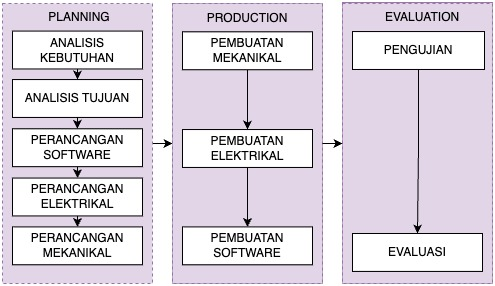
\includegraphics[scale=0.7]{gambar/method_diagram.jpg}
  % Keterangan gambar yang diinputkan
  \caption{Diagram alur penelitian}
  % Label referensi dari gambar yang diinputkan
  \label{fig:Diagram alur penelitian}
\end{figure}

\subsection{Perencanaan (\emph{Planning})}
Pada tahap ini, peneliti melakukan analisis dan perancangan prototipe. Analisis kebutuhan dilakukan untuk mengidentifikasi fitur dan spesifikasi yang diperlukan. Selain itu, analisis tujuan dilakukan untuk menentukan sasaran yang ingin dicapai dengan teknologi yang akan diterapkan. Berdasarkan hasil analisis kebutuhan dan tujuan, dilakukan perancangan prototipe yang mencakup perancangan perangkat lunak (\emph{software}), perancangan elektrikal, dan perancangan mekanikal.

\subsection{Produksi (\emph{Production})}
Tahap produksi mencakup pengembangan robot berdasarkan rencana yang telah dibuat. Pengembangan ini meliputi pembuatan komponen mekanikal, elektrikal, dan perangkat lunak (\emph{software}) sesuai dengan desain yang telah ditetapkan. Setiap komponen robot dikembangkan secara terintegrasi untuk memastikan kesesuaian dan kinerja sistem secara keseluruhan.

\subsection{Evaluasi (\emph{Evaluation})}
Pada tahap evaluasi, dilakukan pengujian secara bertahap untuk memastikan bahwa robot dapat beroperasi sesuai dengan tujuan yang telah ditetapkan. Pertama, dilakukan pengujian sub-sistem untuk memastikan setiap komponen sistem berfungsi dengan baik. Selanjutnya, pengujian terhadap fungsi-fungsi utama robot, seperti navigasi, deteksi \emph{overheat}, dan pengendalian jarak jauh, dilakukan untuk memastikan performa sistem secara keseluruhan. Terakhir, dilakukan pengujian di lingkungan nyata untuk menilai kinerja robot dalam kondisi operasional sesungguhnya. Jika ditemukan kekurangan atau masalah, perbaikan akan dilakukan untuk memastikan kinerja robot optimal dan sesuai dengan tujuan penelitian.


\section{Analisis Sistem}
Analisis dibagi menjadi analisis kebutuhan dan analisis tujuan seperti penjelasan berikut.

\subsection{Analisis Kebutuhan}
Analisis kebutuhan dilakukan melalui pengumpulan data dari studi literatur dan wawancara dengan pihak-pihak terkait. Berdasarkan hasil analisis, beberapa kebutuhan sistem yang harus dipenuhi adalah sebagai berikut:
\begin{enumerate}
  \item Sistem harus mampu mengidentifikasi komponen yang mengalami \emph{overheat} pada gardu listrik dengan menggunakan kamera termal, serta memberikan estimasi posisi dan jenis komponen yang terdeteksi.
  \item Sistem harus mampu melakukan patroli secara otonom di area gardu listrik, mengikuti jalur inspeksi yang telah ditentukan, dan menghindari rintangan fisik yang terdapat pada sekitar robot.
  \item Sistem harus dapat berkomunikasi secara \emph{online} dengan \emph{control station} untuk mengirimkan data posisi dan informasi deteksi robot secara real-time, serta menerima perintah kontrol seperti penetapan rute, jadwal patroli, serta perintah untuk melakukan \emph{wireless emergency stop} apabila terjadi keadaan darurat.
\end{enumerate}

\subsection{Analisis Tujuan}
Berdasarkan hasil analisis kebutuhan adapun tujuan yang ingin dicapai dalam pengembangan sistem ini adalah sebagai berikut:
\begin{enumerate}
  \item Mengembangkan sistem \emph{computer vision} untuk mendeteksi dan mengidentifikasi komponen yang mengalami \emph{overheat} menggunakan kamera termal. Sistem ini juga harus mampu memperkirakan posisi dan jenis komponen yang terdeteksi mengalami \emph{overheat}.
  \item Merancang dan mengimplementasikan sistem navigasi otonom pada robot, sehingga robot dapat melakukan patroli secara mandiri di area gardu listrik, menghindari rintangan fisik, dan mengikuti jalur inspeksi yang telah ditentukan. Sistem navigasi ini harus beroperasi dengan stabil dan akurat di lingkungan yang memiliki gangguan elektromagnetik serta interferensi dari peralatan listrik.
  \item Merancang dan membangun \emph{control station} yang dapat memantau lokasi robot dan hasil deteksi \emph{overheat} secara \emph{real-time}. Sistem ini harus dapat mengirim perintah kontrol \emph{emergency stop} secara \emph{wireless} ke robot. Selain itu, sistem harus dapat beroperasi secara online dan dapat diakses dari jarak jauh.
\end{enumerate}

\section{Desain Mekanikal}
Penelitian ini menggunakan robot \emph{quadruped legged} tipe \emph{DeepRobotics Jueying Lite 3 Pro} sebagai basis robot. Modifikasi dilakukan dengan menambahkan plat aluminium pada bagian atas robot sebagai tempat peletakan komponen. Plat aluminium ini dilapisi dengan cat isolator untuk mencegah terjadinya konduksi listrik, mengingat robot akan beroperasi di area gardu listrik.  Komponen tambahan yang dipasang meliputi kamera termal dan sensor LiDAR yang diletakkan di bagian depan robot, serta modul GPS, \emph{switch}, dan modem yang ditempatkan di dalam \emph{electrical box}. \emph{Electrical box} ini dirancang menggunakan teknologi \emph{3D printing} sebagai pelindung komponen elektronik dari benturan dan kerusakan akibat lingkungan eksternal.Desain mekanikal robot dirancang sedemikian rupa agar komponen tambahan dapat terpasang dengan aman tanpa mengganggu pergerakan robot. Seperti pada gambar \ref{fig:DesignMekanikalRobot},

\begin{figure}[H]
  \centering
  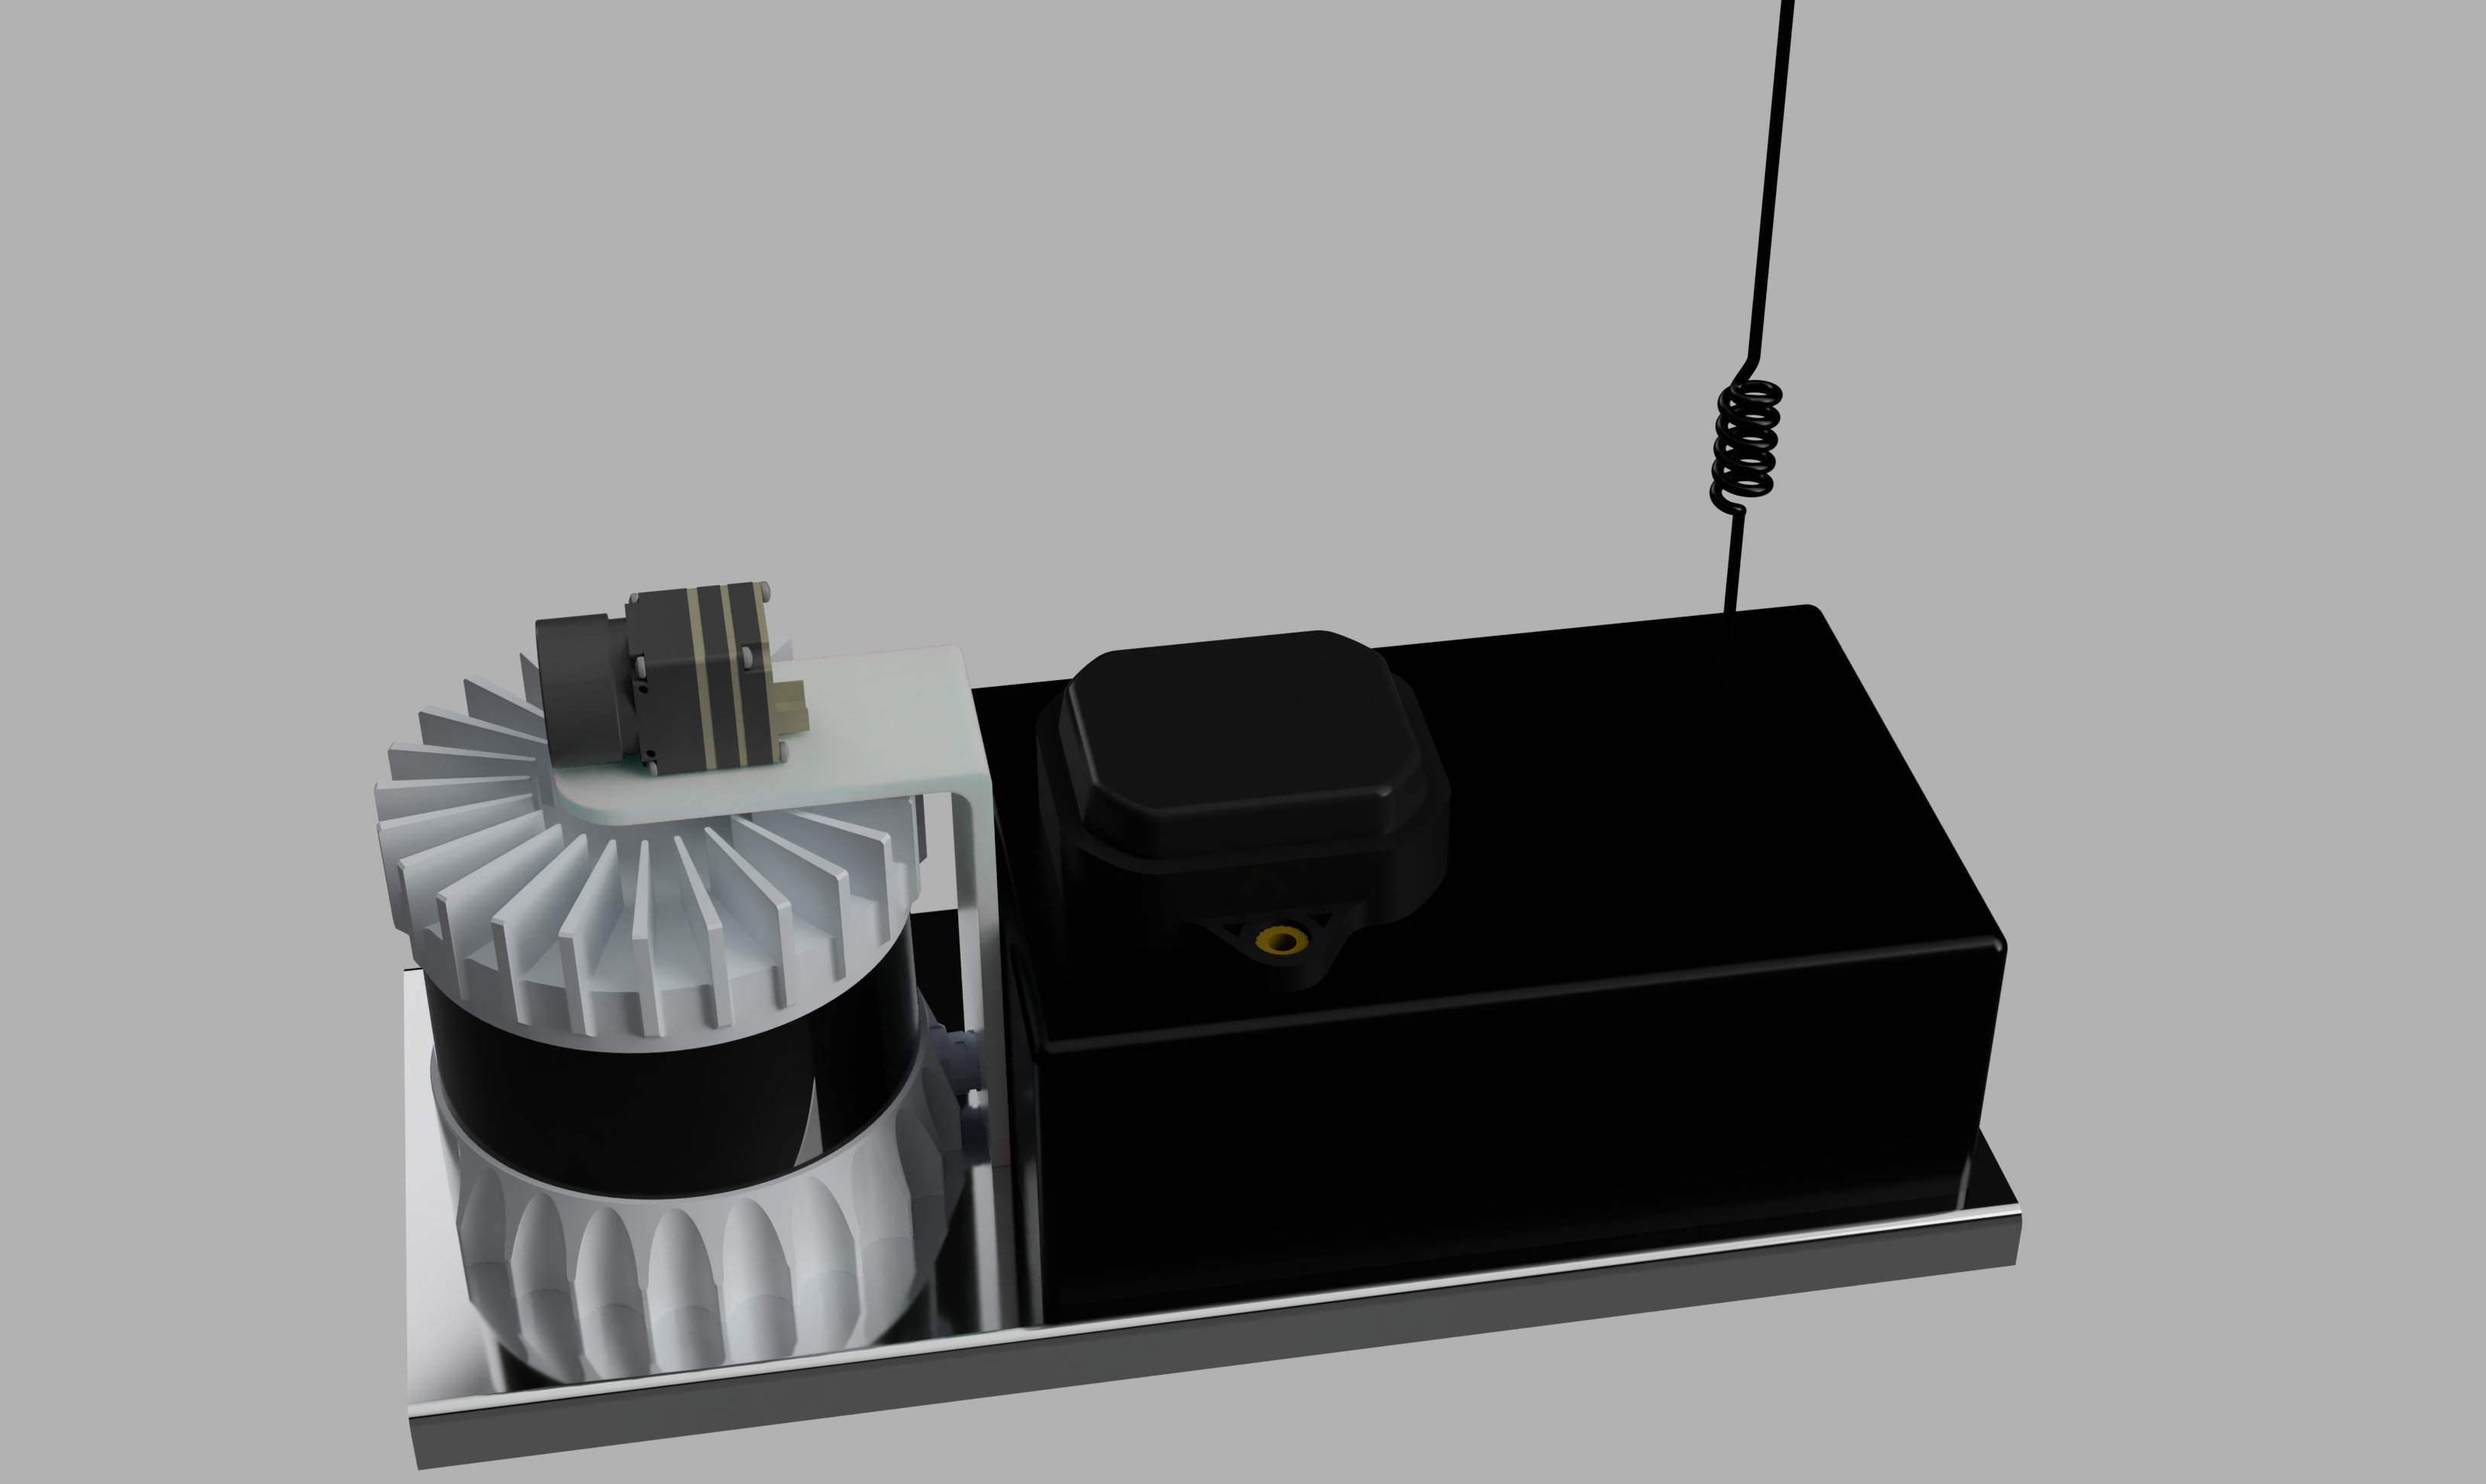
\includegraphics[scale=0.11]{gambar/mechanical_design.png}
  \caption{Desain komponen mekanikal robot}
  \label{fig:DesignMekanikalRobot}
\end{figure}

Penempatan sensor LiDAR di bagian atas robot memungkinkan sensor untuk memperoleh pandangan yang lebih luas, sedangkan kamera termal ditempatkan di posisi strategis untuk mendeteksi perubahan suhu pada komponen gardu listrik. \emph{Electrical box} dipasang di bagian belakang robot untuk mengoptimalkan distribusi berat dan memastikan kestabilan robot.


